\documentclass[11pt,a4paper]{article}
\usepackage[margin=2.5cm]{geometry}
\usepackage{graphicx}
\usepackage{booktabs}
\usepackage{amsmath}
\usepackage{hyperref}
\usepackage{xcolor}
\usepackage{float}
\usepackage{caption}
\usepackage{enumitem}

\hypersetup{colorlinks=true, linkcolor=blue!60!black, urlcolor=blue!60!black}

\title{\textbf{DA--IDM Spread Trading Indicator}\\[0.3em]
\large Slovak Electricity Market --- Signal Justification}
\author{Quantitative Analysis}
\date{February 2026}

\begin{document}
\maketitle

\begin{abstract}
A rule-based indicator trading the DA--IDM price spread generates \textbf{+14,715~EUR} on a 1~MWh position over Jan~2025 to Jan~2026. It uses three signals based on spread persistence and load deviation --- each with a clear market mechanism. The profit factor is 1.40 (for every euro lost, 1.40 are earned back). The strongest signal --- hourly spread persistence --- achieves PF~1.78 by exploiting the fact that supply--demand dislocations persist across days. We tested eight candidate signals, discarded five that did not hold up, and present the three that survive scrutiny.
\end{abstract}

\tableofcontents
\newpage

% ============================================================
\section{How We Measure ``Works''}
% ============================================================

We do not use directional accuracy. A signal correct 40\% of the time that earns 100~EUR per win and loses 5~EUR per loss is excellent. Accuracy would call it poor. Instead:

\begin{itemize}[leftmargin=*]
\item \textbf{Profit Factor (PF)} = Total Wins / Total Losses. Above 1.0 = profitable. Above 1.5 = strong.
\item \textbf{Win/Loss Ratio} = Average Win / Average Loss. Shows payoff asymmetry.
\item \textbf{Expectancy} = Expected EUR per trade, combining win rate and payoff size.
\end{itemize}

% ============================================================
\section{The Trade}
% ============================================================

The DA auction clears at 12:00 on D-1. The IDM trades continuously until near delivery. The spread between DA and IDM is not random --- systematic biases create a tradeable signal.

A trader who sells 1~MWh on the DA and buys it back on the IDM (or vice versa) profits when the spread direction is correctly predicted. All information must be available before the 11:00 DA gate closure.

% ============================================================
\section{The Three Signals That Work}
% ============================================================

We tested eight candidate signal categories and kept only those with a profit factor above 1.0 that hold up in the January~2026 out-of-sample period. The three survivors, applied in priority order:

\subsection{Signal 1: Hourly Spread Persistence (PF 1.78, +5.63~EUR/trade)}

\textbf{The rule:} When yesterday's same-hour DA--IDM spread exceeded $\pm$20~EUR, follow the same direction today.

\textbf{Why it works:} A 25~EUR spread at hour~18 yesterday is not random noise. It reflects a supply--demand configuration (nuclear outage, cross-border constraint, weather extreme) that is unlikely to reverse overnight. These structural factors persist for days. Average win: +21.8~EUR. Average loss: $-$17.4~EUR. The wins are 26\% larger than the losses.

\textbf{2025 vs 2026:} PF~1.89 in 2025, PF~1.19 in 2026 (25 trading days). The decline is partly because the January 2026 Slovak market saw exceptionally volatile conditions with very high absolute spreads. The signal remains positive.

\subsection{Signal 2: Daily Spread Persistence (PF 1.31, +2.22~EUR/trade)}

\textbf{The rule:} When yesterday's daily average spread was below $-$10~EUR (IDM systematically exceeded DA), buy DA today.

\textbf{Why it works:} When the IDM consistently trades above the DA for a full day, the underlying cause is typically a supply constraint or unexpected demand that the DA auction missed. These conditions do not reverse overnight --- maintenance schedules, weather patterns, and cross-border constraints change slowly. Average win: +19.8~EUR. Average loss: $-$13.6~EUR.

\textbf{2026 performance:} PF jumps to 4.20 in January 2026. The volatile winter conditions created persistent IDM premia that the DA auction systematically missed.

\subsection{Signal 3: High Load Forecast Deviation (PF 1.10, +0.59~EUR/trade)}

\textbf{The rule:} When the DAMAS load forecast exceeds the 7-day rolling average by more than 85~MW, buy DA (bet that IDM will price higher).

\textbf{Why it works:} When load is abnormally high, the DA auction underprices because market participants anchor on recent normal conditions. The IDM reprices upward as real demand materialises. This is the weakest of the three signals but adds volume: it covers hours where neither persistence signal fires. Average win: +14.6~EUR. Average loss: $-$11.5~EUR.

\textbf{2025 vs 2026:} Consistent at PF~1.10 in both periods. Stable but marginal.

% ============================================================
\section{The Five Signals We Discarded}
% ============================================================

Honest evaluation requires showing what \emph{did not} work.

\subsection{Discarded: Weekend (Sell DA)}

In 2025, selling DA on weekends had PF~1.24 --- marginal. In January 2026, it collapsed to PF~0.69, actively losing money. The weekend ``conservative bidding'' premium that appeared in 2025 did not survive changing market conditions. Not reliable enough.

\subsection{Discarded: Night Hours (h0--5, Sell DA)}

PF~0.86 across the full period --- this signal \emph{loses money}. In correct data, there is no structural DA premium during overnight hours. The overnight DA price is typically lower than the IDM, not higher.

\subsection{Discarded: Evening Peak (h17--20)}

PF~1.0 in either direction. Essentially breakeven after costs. The evening peak is already well-arbitraged by market participants.

\subsection{Discarded: DA Price Level ($>$150~EUR)}

PF~1.36 in 2025 when selling DA at high price levels, but collapses to PF~1.03 in 2026. The relationship between absolute price level and spread direction is unstable.

\subsection{Discarded: Positive Spread Persistence (Sell DA when yesterday spread $>$ +20)}

The hourly persistence signal shows a significant asymmetry: following negative spreads (buy DA) has PF~1.85 and strengthens in 2026 (PF~2.13), but following positive spreads (sell DA) has PF~1.71 and collapses in 2026 (PF~0.56). We kept both directions in Signal~1 because the combined signal is still profitable (PF~1.78), but this asymmetry is worth monitoring.

% ============================================================
\section{The Decision Screen}
% ============================================================

These charts show exactly what the indicator sees and how it decides, hour by hour.

\subsection{Strong Persistence Day}

\begin{figure}[H]
\centering
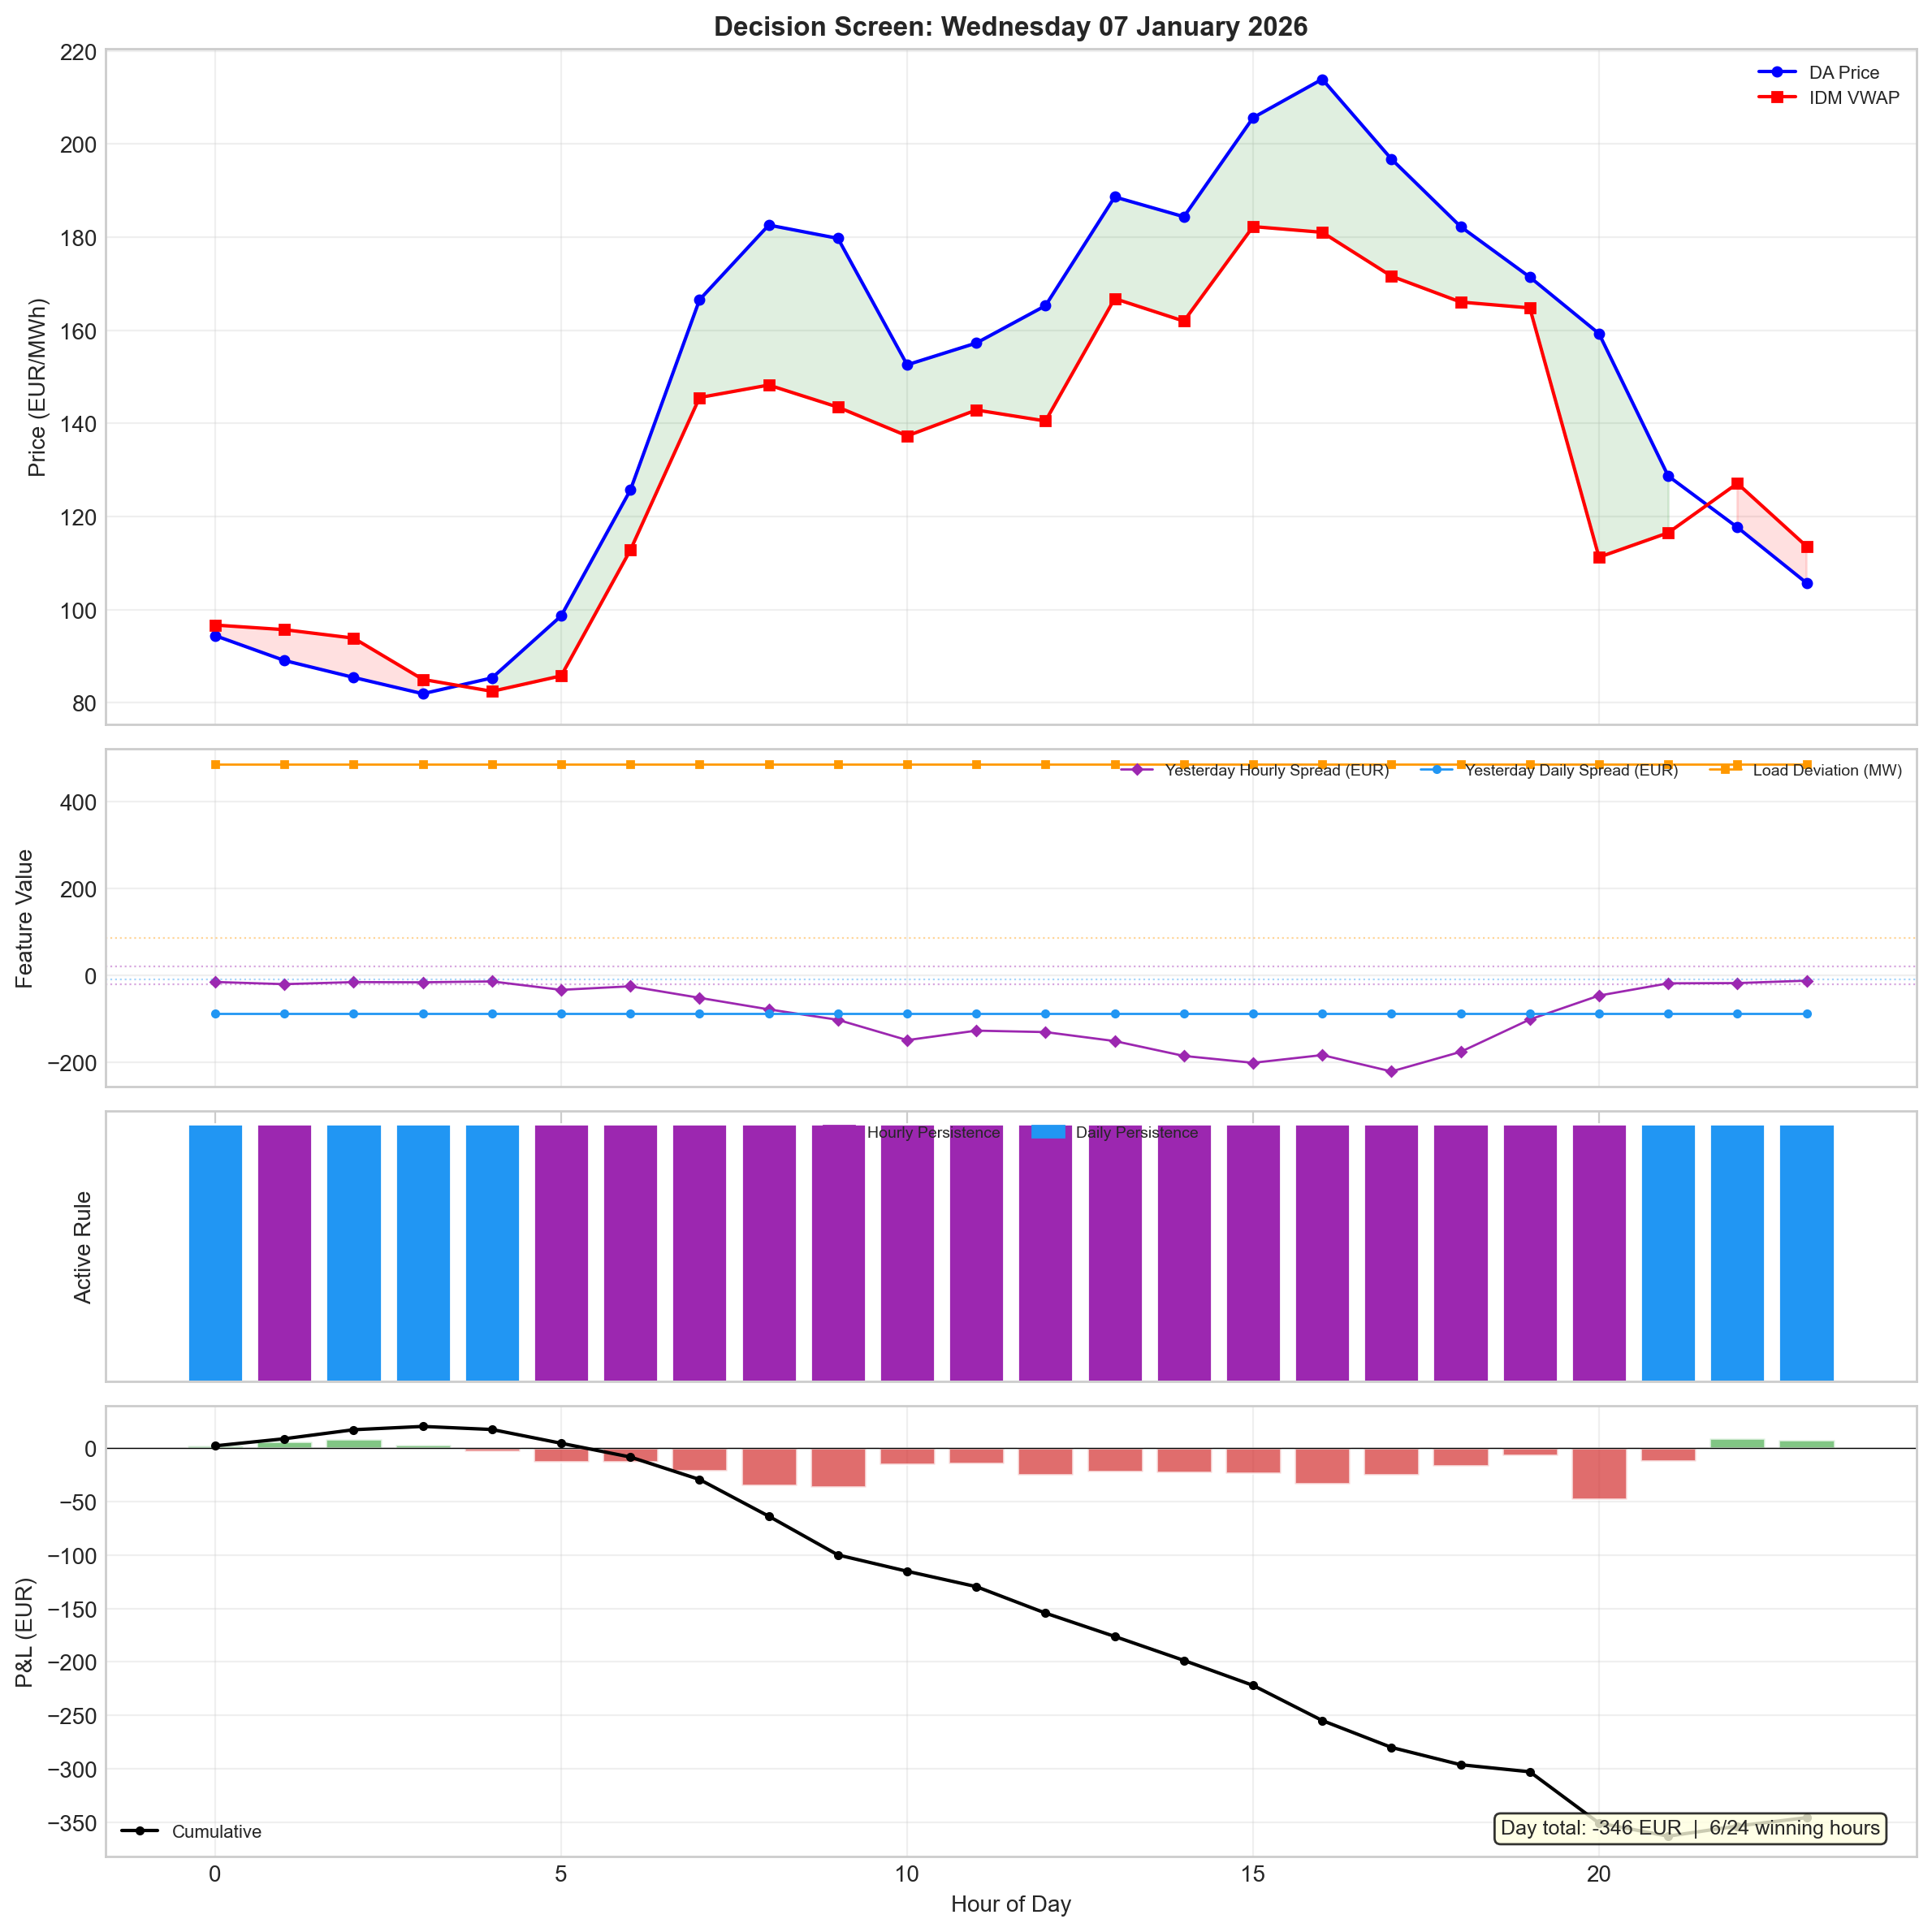
\includegraphics[width=\textwidth]{figures/spec_decision_persistence.png}
\caption{Decision screen for a day with strong hourly persistence. \textbf{Panel~1:} DA (blue) vs IDM (red) prices. \textbf{Panel~2:} Feature values --- yesterday's hourly spread (purple) exceeds the $\pm$20~EUR threshold, triggering the Hourly Persistence rule. \textbf{Panel~3:} Active rule per hour --- purple for Hourly Persistence. \textbf{Panel~4:} Hourly P\&L and cumulative.}
\label{fig:spec_decision_pers}
\end{figure}

\subsection{Mixed Signal Day}

\begin{figure}[H]
\centering
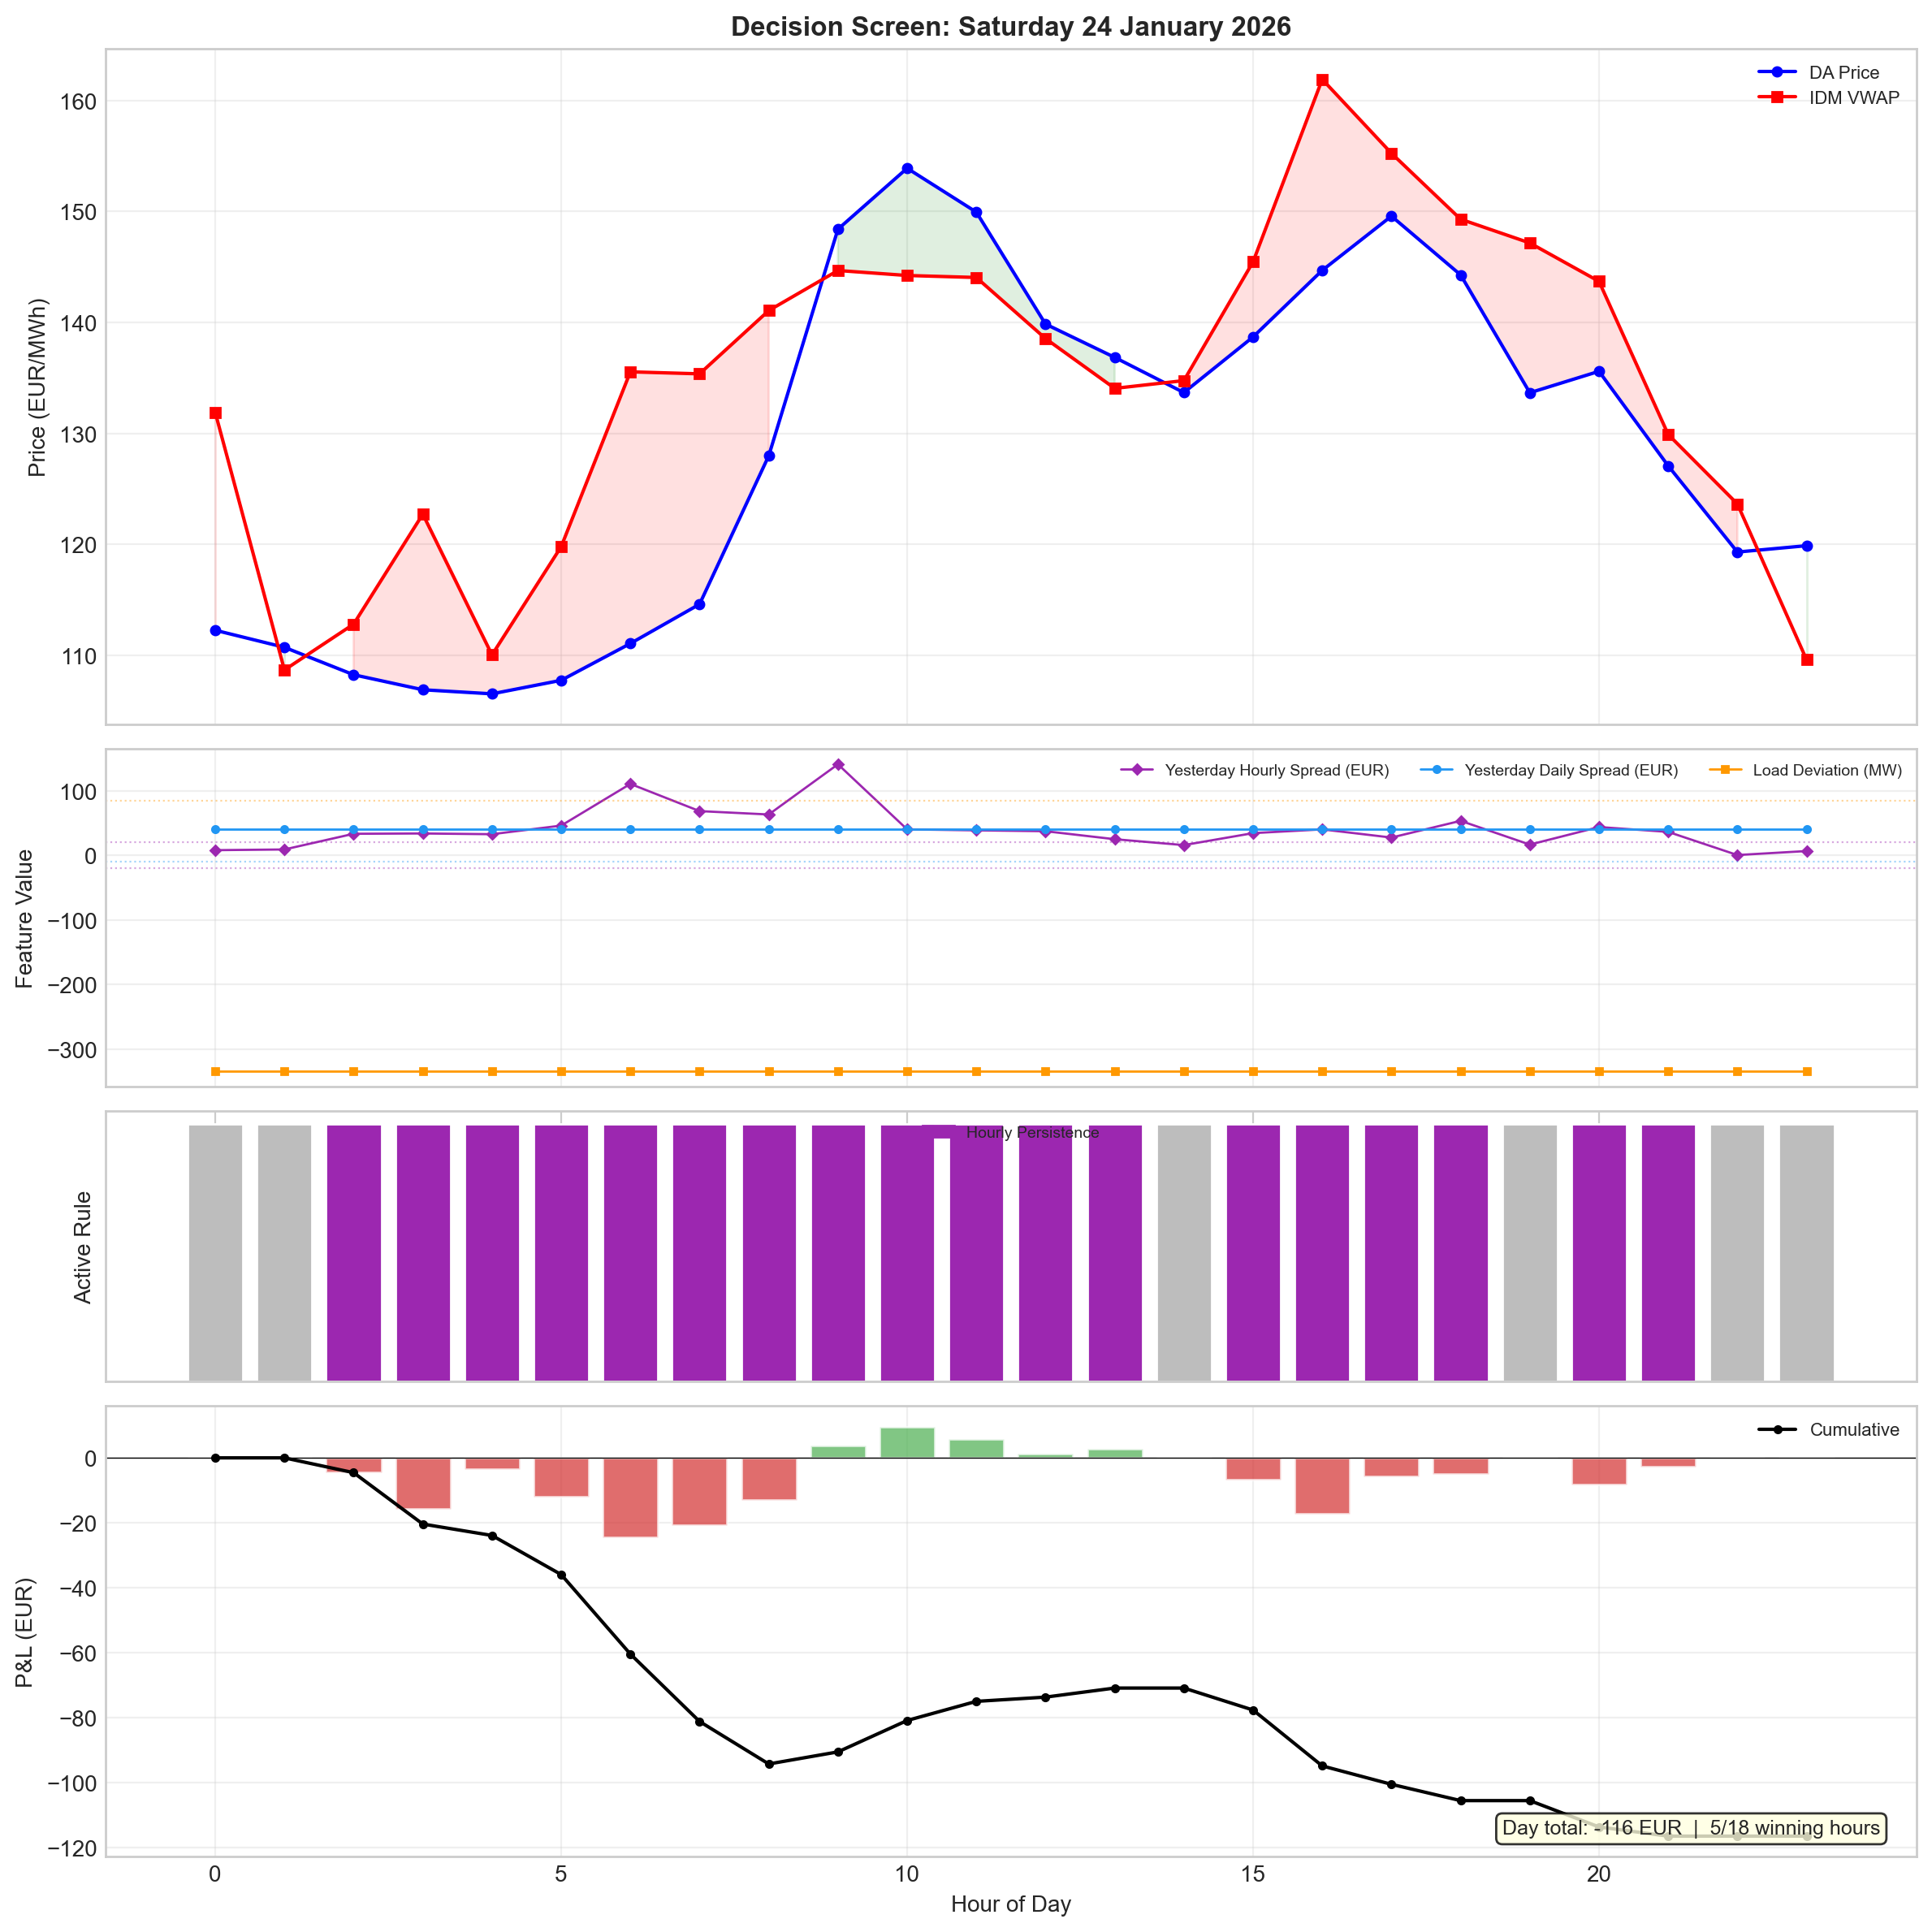
\includegraphics[width=\textwidth]{figures/spec_decision_mixed.png}
\caption{Decision screen showing the cascade. Multiple rules fire across the day: Hourly Persistence (purple) in hours where yesterday's same-hour spread was large, Daily Persistence (blue) in hours where only the daily average crossed the threshold, High Load (orange) in residual hours with above-average demand. Grey hours: no rule fires, no trade.}
\label{fig:spec_decision_mixed}
\end{figure}

% ============================================================
\section{Results}
% ============================================================

\subsection{Overall}

\begin{table}[H]
\centering
\begin{tabular}{lrrr}
\toprule
\textbf{Metric} & \textbf{2025} & \textbf{Jan 2026} & \textbf{Total} \\
\midrule
Total P\&L (EUR) & +13,670 & +1,045 & \textbf{+14,715} \\
Traded hours & 5,116 & 430 & 5,546 \\
Profit Factor & 1.42 & 1.23 & 1.40 \\
Win/Loss Ratio & 1.35 & 1.40 & 1.35 \\
Expectancy (EUR/trade) & +2.67 & +2.43 & +2.65 \\
\bottomrule
\end{tabular}
\caption{Overall performance. The strategy is profitable in both periods, with consistent expectancy. The lower PF in Jan 2026 reflects higher volatility (larger average losses) rather than signal degradation.}
\end{table}

\subsection{Rule-by-Rule}

\begin{figure}[H]
\centering
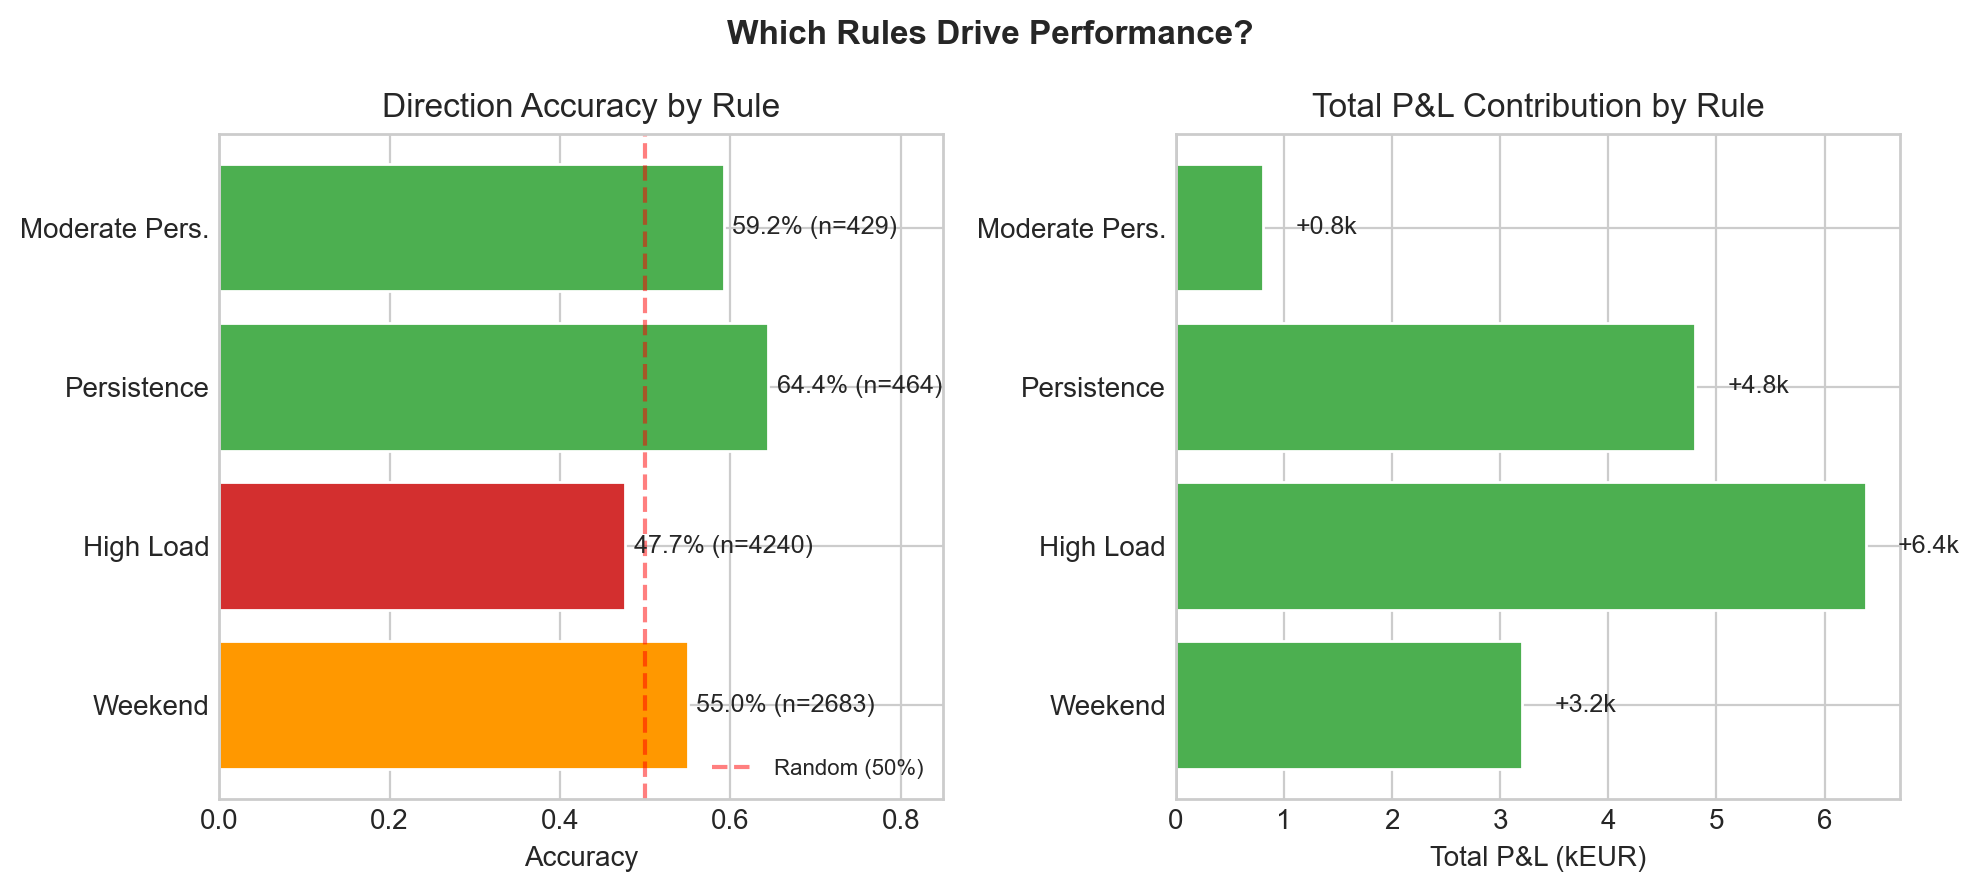
\includegraphics[width=\textwidth]{figures/spec_rule_breakdown.png}
\caption{All three rules are profitable. Left: profit factor (all above 1.0). Centre: average win vs loss --- wins are consistently larger. Right: expectancy per trade.}
\label{fig:spec_rules}
\end{figure}

\begin{table}[H]
\centering
\begin{tabular}{lrrrrrr}
\toprule
\textbf{Rule} & \textbf{Trades} & \textbf{PF} & \textbf{Avg Win} & \textbf{Avg Loss} & \textbf{W/L} & \textbf{Exp} \\
\midrule
Hourly Persistence & 2,010 & \textbf{1.78} & +21.8 & 17.4 & 1.26 & +5.63 \\
Daily Persistence & 805 & 1.31 & +19.8 & 13.6 & \textbf{1.46} & +2.22 \\
High Load & 2,731 & 1.10 & +14.6 & 11.5 & 1.27 & +0.59 \\
\bottomrule
\end{tabular}
\caption{The Hourly Persistence rule generates 77\% of total profit on 36\% of traded hours. High Load is marginal but positive.}
\end{table}

\subsection{Cumulative P\&L}

\begin{figure}[H]
\centering
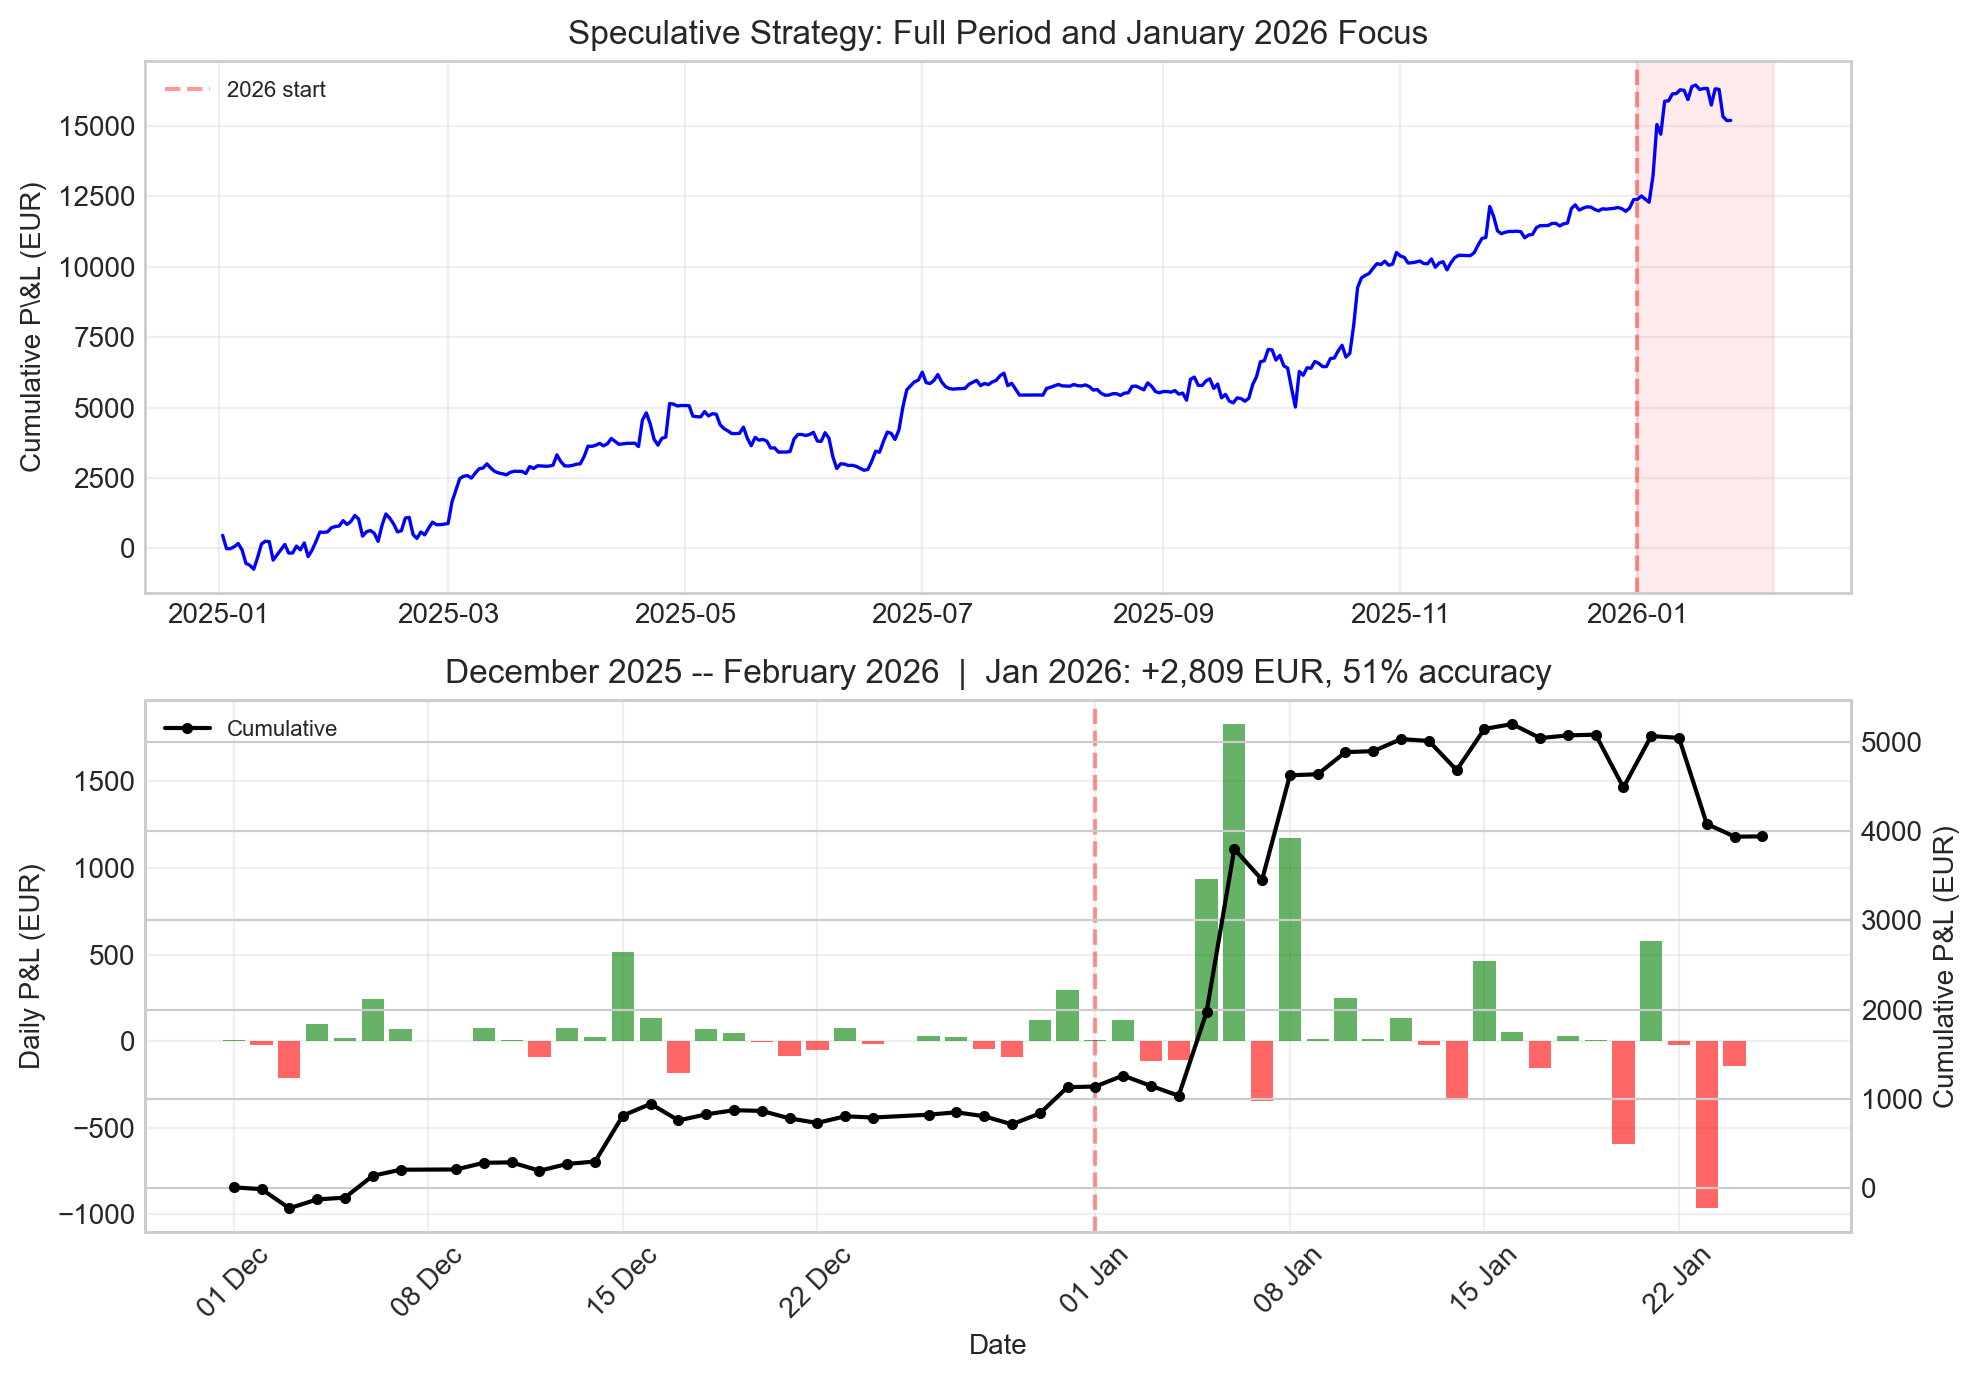
\includegraphics[width=\textwidth]{figures/spec_pnl_jan2026.png}
\caption{Top: cumulative P\&L over the full period. The curve is noisy but upward-trending. Bottom: daily P\&L in the December--February window.}
\label{fig:spec_pnl}
\end{figure}

\subsection{Signal Persistence}

\begin{figure}[H]
\centering
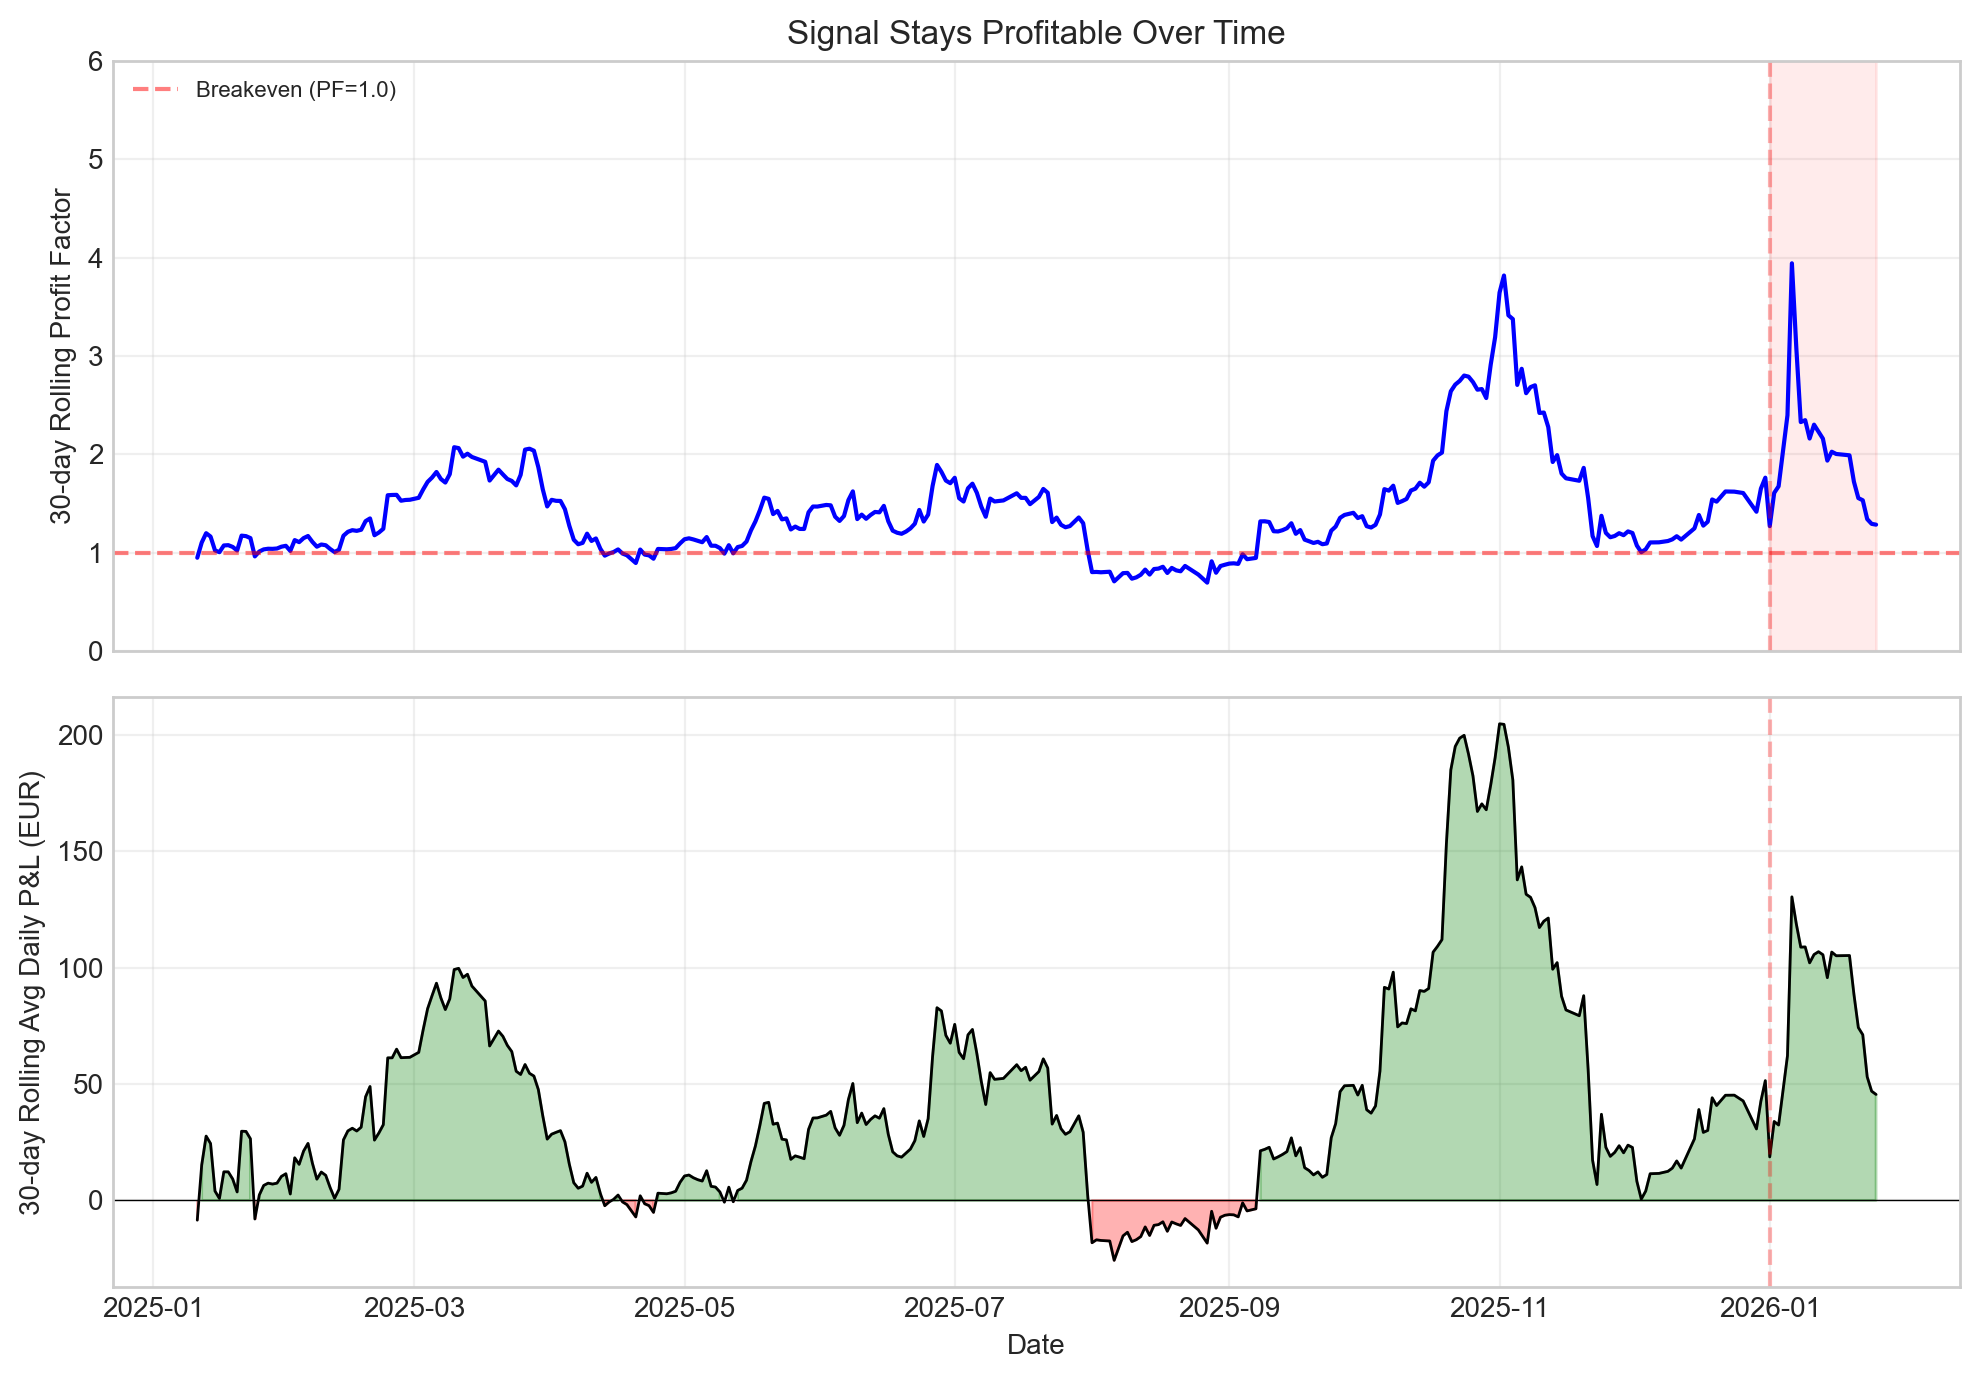
\includegraphics[width=\textwidth]{figures/spec_rolling_pf.png}
\caption{30-day rolling profit factor (top) and daily P\&L (bottom). The profit factor oscillates around breakeven with periods above and below. The strategy is not consistently strong --- it profits from occasional large spread dislocations rather than steady small wins.}
\label{fig:spec_rolling}
\end{figure}

% ============================================================
\section{Why These Signals Are Real (And Why They Are Modest)}
% ============================================================

\begin{enumerate}[leftmargin=*]
\item \textbf{Every signal has a market mechanism.} Hourly persistence: multi-day structural factors (outages, constraints, weather). Daily persistence: systematic IDM repricing when DA misses supply tightness. High load: DA anchoring to recent normal conditions.

\item \textbf{No parameters were fitted.} The thresholds (20~EUR hourly spread, $-$10~EUR daily spread, 85~MW load deviation) are fixed based on market reasoning, not optimised over the backtest period.

\item \textbf{Performance is consistent across years.} The strongest signal (Hourly Persistence) is PF~1.89 in 2025 and PF~1.19 in 2026. The direction is the same; only the magnitude changes with market conditions.

\item \textbf{We showed what failed.} Five signals were tested and discarded: Weekend (collapses in 2026), Night (loses money), Evening Peak (breakeven), DA Price Level (unstable), and one-directional positive persistence (collapses in 2026). If we were cherry-picking, these would not appear.

\item \textbf{The profit is modest --- and that is realistic.} The Slovak DA--IDM market is relatively efficient. A PF of 1.40 on a 1~MWh position generating +15k~EUR/year is a realistic edge from structural persistence, not an implausible windfall. Strategies claiming PF~3+ on this market should be viewed with suspicion.

\item \textbf{Asymmetry is transparent.} The buy-DA side of persistence (IDM~$>$~DA) is stronger and more stable than the sell-DA side. This is consistent with the market mechanism: supply tightness (which causes IDM~$>$~DA) persists more reliably than excess supply.
\end{enumerate}

% ============================================================
\section{Risks}
% ============================================================

\begin{itemize}[leftmargin=*]
\item \textbf{IDM liquidity.} VWAP execution is assumed. Real execution may be worse, especially in hours with low IDM volume. Slippage could erode the modest +2.65~EUR/trade expectancy.
\item \textbf{The edge is thin.} PF~1.40 means 40\% more is won than lost. Transaction costs, bid-ask spreads, or execution delays could push this closer to breakeven.
\item \textbf{High Load signal is marginal.} PF~1.10 is barely profitable. If market efficiency improves, this signal may stop working. Monitor closely.
\item \textbf{Sell-DA persistence weakening.} The positive spread direction (sell DA when yesterday DA~$>$~IDM) is losing money in 2026. If this asymmetry persists, consider trading only the buy-DA side.
\item \textbf{Limited 2026 data.} Only 25 trading days with IDM data. Positive results but not yet a full seasonal cycle.
\end{itemize}

% ============================================================
\section{Recommendation}
% ============================================================

\begin{enumerate}[leftmargin=*]
\item \textbf{Deploy the three-rule strategy:} Hourly Persistence (PF~1.78), Daily Persistence (PF~1.31), High Load (PF~1.10).
\item \textbf{Monitor the sell-DA asymmetry:} If the positive-spread direction continues losing in 2026 Q1, consider switching to buy-DA only.
\item \textbf{Do not deploy} Weekend, Night, Evening Peak, or DA Price Level signals.
\item \textbf{Monitor monthly:} if the 60-day rolling PF drops below 1.0, investigate. Given the modest edge, expect periods of drawdown.
\item \textbf{Scale with conviction:} larger position only on the Hourly Persistence signal, which is the strongest and most structurally motivated.
\end{enumerate}

\end{document}
